\documentclass{article}
\usepackage{graphicx} % Required for inserting images
\usepackage{amsmath}
\usepackage{amssymb}
\usepackage{pdfpages}

%テキストの表示領域の調節
\setlength{\textwidth}{\paperwidth}
\addtolength{\textwidth}{-40truemm}
\setlength{\textheight}{\paperheight}
\addtolength{\textheight}{-45truemm}

%余白の調節
\setlength{\topmargin}{-10.4truemm}
\setlength{\evensidemargin}{-5.4truemm}
\setlength{\oddsidemargin}{-5.4truemm}
\setlength{\headheight}{17pt}
\setlength{\headsep}{10mm}
\addtolength{\headsep}{-17pt}
\setlength{\footskip}{5mm}

\title{Ecomonmetrics II HW1}
\author{29-246004 Kosuke IGARASHI}
\date{June 24 2025}

\begin{document}

\maketitle

\section{Exercise 14.14}
Assume $e_t$ and $u_t$ is white noise process.\\ 
We have
\begin{center}
           \begin{align*}
             Y_t&=X_t+e_t\\
             &=\alpha X_{t-1}+u_t+e_t\\
             &=\alpha (Y_{t-1}-e_{t-1})+u_t+e_t\\
             &=\alpha Y_{t-1}+u_t+e_t-\alpha e_{t-1}\\
             &=\alpha Y_{t-1}+w_t
            \end{align*}
           \end{center}

where $w_t=u_t+e_t-\alpha e_{t-1}$\\
$e_t$ and $u_t$ are mutually independent i.i.d, so {$w_t$} is strictly stationary.\\
Because $e_t$ and $u_t$ is white noise process,\\ 
$$
\begin{aligned}
v\left(w_t\right)= & v\left(u_t+e_t-\alpha e_{t-1}\right) \\
= & v\left(u_t\right)+v\left(e_t\right)+\alpha^2 v\left(e_{t-1}\right)+2 \operatorname{cov}\left(u_t, e_t\right) \\
& -2 \alpha \operatorname{cov}\left(e_t, e_{t-1}\right)-2 \alpha \operatorname{cov}\left(u_t, e_{t-1}\right) \\
= & v\left(u_t\right)+v\left(e_t\right)+\alpha^2 v\left(e_{t-1}\right)<\infty
\end{aligned}
$$

$$
\operatorname{cov}\left(w_t, w_{t-s}\right)
=\left\{\begin{array}{ccc}
-\alpha v\left(e_{t-1}\right) & \neq 0 & s=1 \\
0 & & s \geq 2
\end{array}\right.
$$
Therefore  ${w_t}$  is white noise and $Y_t$ is an ARMA(1,1) process.

\section{Exercise 14.15}
    Consider the AR(1) process \(Y_t =\alpha_0 + \alpha_1 Y_{t-1} + e_t\).
    Since this is transformed into \((1-\alpha_1 L)Y_t=\alpha_0 + e_t\), we get the MA representation of \(Y_t\) as
    \[
    Y_t = (1-\alpha_1 L)^{-1}(\alpha_0+e_t)
         =\frac{\alpha_0}{1-\alpha_1} + \sum_{j=0}^\infty \alpha_1^j e_{t-j}.
    \]
    
    Because \(|\alpha_1|<1\), the coefficients satisfy \(\sum_{j=0}^\infty \alpha_1^{2j}<\infty\). Hence
    \begin{align*}
        E[Y_t]
        =E\left[\frac{\alpha_0}{1-\alpha_1} + \sum_{j=0}^\infty \alpha_1^j e_{t-j}\right]
        =\frac{\alpha_0}{1-\alpha_1} + \sum_{j=0}^\infty \alpha_1^j E[e_{t-j}]
        =\frac{\alpha_0}{1-\alpha_1},\\
        Var(Y_t) = Var\left(\sum_{j=0}^\infty \alpha_1^j e_{t-j}\right)=\sum_{j=0}^\infty \alpha_1^{2j} Var(e_{t-j})=\sigma^2 \sum_{j=0}^\infty \alpha_1^{2j}=\frac{\sigma^2}{1-\alpha_1^2}.
    \end{align*}

    Define the moment--generating function,
    \[
        M_S(t) \;:=\; E\!\bigl[e^{tS}\bigr],
        \quad t\in \mathbb{R}.
    \]
    Using independence, factor the expectation:
    \[
    \begin{aligned}
        M_S(t)
        = E\!\Bigl[\exp\bigl\{t\sum_{j=0}^{\infty}\alpha_1^{\,j}e_{t-j}\bigr\}\Bigr]
        = \prod_{j=0}^{\infty} E\!\bigl[e^{\,t\alpha_1^{\,j}e_{t-j}}\bigr].
    \end{aligned}
    \]
    Each term is the MGF of a normal variable with mean \(0\) and variance
    \(\alpha_1^{2j}\sigma^{2}\):
    \[
        E\!\bigl[e^{\,t\alpha_1^{\,j}e_{t-j}}\bigr]
        = \exp\!\Bigl\{\tfrac12 t^{2}\alpha_1^{2j}\sigma^{2}\Bigr\}.
    \]
    Hence
    \[
        M_S(t)
        = \prod_{j=0}^{\infty}
          \exp\!\Bigl\{\tfrac12 t^{2}\alpha_1^{2j}\sigma^{2}\Bigr\}
        = \exp\!\Bigl\{\tfrac12 t^{2}\sigma^{2}
            \sum_{j=0}^{\infty}\alpha_1^{2j}\Bigr\}.
    \]
    Because \(|\alpha_1|<1\), the geometric series converges:
    \(
        \sum_{j=0}^{\infty}\alpha_1^{2j} = 1/(1-\alpha_1^{2}).
    \)
    Thus
    \[
        M_S(t)
        = \exp\!\Bigl\{\tfrac12 t^{2}\sigma^{2}/(1-\alpha_1^{2})\Bigr\},
    \]
    which is precisely the MGF of the normal distribution
    \(N\!\bigl(0,\sigma^{2}/(1-\alpha_1^{2})\bigr)\).
    Therefore
    \[
        S \;\sim\; N\!\Bigl(0,\;\sigma^{2}/(1-\alpha_1^{2})\Bigr).
    \]
    
    Finally,
    \[
        Y_t
        = \frac{\alpha_0}{1-\alpha_1} + S
        \;\sim\;
        N\!\Bigl(
            \tfrac{\alpha_0}{1-\alpha_1},
            \tfrac{\sigma^{2}}{1-\alpha_1^{2}}
          \Bigr),
    \]
    so the marginal distribution of the stationary AR(1) process is Gaussian
    with the stated mean and variance.

\section{Exercise 14.18}
\textbf{Please refer to the end of this document.}

\section{Exercise 16.1}

\begin{itemize}
  \item[(a) ] 
  \begin{align*}
    S_t &= e_t + e_{t-1} + \cdots + e_1 + S_0 \\
    & = e_t + e_{t-1} + \cdots + e_1.
  \end{align*}
  Since $e_t$ is i.i.d, $E[e_t]=0$ and $V(e_t)=\sigma^2$,
  \begin{align*}
      E[S_t]=E[e_t+t_t-1+\cdots+e_1]=0\\
      V(S_t)=V(e_t+t_t-1+\cdots+e_1)=t\sigma^2
  \end{align*}

  \item[(b) ] 
  \begin{equation*}
      Y_t = \frac{S_t-E[S_t]}{\sqrt{V(S_t)}}=\frac{S_t}{\sigma\sqrt{t}}
  \end{equation*}
  Therefore,
  \begin{align*}
      Cov(T_t,Y_{t-j}) &= Cov(\frac{S_t}{\sigma\sqrt{t}},\frac{S_{t-j}}{\sigma\sqrt{t-j}})\\
      &= E[\frac{S_tS_{t-j}}{\sigma^2\sqrt{t(t-j)}}] \quad (\because E[S_t]=0)\\
      &= \frac{E[(e_t+\cdots+e_1)(e_{t-j}+\cdots+e_1)]}{\sigma^2\sqrt{t(t-j)}} \\
      &= \frac{(t-j)\sigma^2}{\sigma^2\sqrt{t(t-j)}} \quad (\because E[e_te_s]=0,  \forall t\neq s) \\
      &= \sqrt{\frac{t-j}{t}}
  \end{align*}
  Thus $Y_t$ is not stationary since this depends on $t$.
  
  \item[(c) ] Assume $\delta>0$.
  \begin{equation*}
      Y_{\lfloor nr \rfloor}=\frac{S_{\lfloor nr\rfloor}}{\sigma\sqrt{\lfloor nr\rfloor}}=\frac{\sum^{\lfloor nr\rfloor}_{s=1}e_s}{\sigma\sqrt{\lfloor nr\rfloor}}
  \end{equation*}
  Since $\lfloor nr\rfloor\rightarrow \infty$ as $n\rightarrow\infty$ because $r\in[\delta,1]$, and $e_t$ follows i.i.d $(0,\sigma^2)$,
  by CLT
  \begin{align*}
      \frac{\sum^{\lfloor nr\rfloor}_{s=1}e_s}{\sqrt{\lfloor nr\rfloor}}\xrightarrow{\mathrm{d}} N(0,\sigma^2)
  \end{align*}
  and then,
  \begin{equation*}
      Y_{\lfloor nr\rfloor}=\frac{\sum^{\lfloor nr\rfloor}_{s=1}e_s}{\sigma\sqrt{\lfloor nr\rfloor}}\xrightarrow{\mathrm{d}}N(0,1).
  \end{equation*}
\end{itemize}

\section{Exercise 16.4}
\subsection{(a)}
Since $e_t$ is i.i.d, $Y_t=e_t$ is i.i.d and that stationary process.
In addition, $\forall j>0, \gamma_j=0$ holds. Thus, as $n\rightarrow\infty$, the long run variance is
\begin{align*}
    nVar(\frac{1}{n}\sum_{t=1}^nY_t)&\rightarrow\gamma_0+2\sum_{j=1}^{\infty}\gamma_j\\
    &=\gamma_0>0
\end{align*}
Hence, $Y_t$ is $I(0)$ process.
\subsection{(b)}
Let $\phi(Y_t,Y_{t-1})=Y_t-Y_{t-1}$. Because $Y_t$ is i.i.d, it is also strictly stationary process. Since $\phi$ is measurable and $X_t = \phi(Y_t,Y_{t-1})$, $X_t$ is also strictly stationary process.
Moreover, because $e_t$ is i.i.d, we have $\forall t\neq j,\  E(e_t)=E(e_j), Var(e_t)=Var(e_j)$, and 
\begin{align*}
    E[X_t]&=E[e_t]+E[e_{t-1}]=0\\
    Cov(X_t,X_{t-j})&=Cov(e_t-e_{t-1},e_{t-j}-e_{t-j-1})\\
    &=E[(e_t-e_{t-1})(e_{t-j}-e_{t-j-1})]\\
    &=\begin{cases}
        2(E[e_t^2]-E[e_t]^2)=2Var(e_t) & \text{when}\ j=0,\\
        E[e_t]^2-E[e_t^2]=-Var(e_t) & \text{when}\ j=1,\\
        0 & \text{when }j\ge2
    \end{cases}
\end{align*}
Since $E(X_t)$ nor $\forall j>0, Cov(X_t,X_{t-j})$ doesn't depends on t, $X_t$ is weekly stationary process.
The long run variance is
\begin{align*}
 nVar\left(\frac{1}{n}\sum_{t=1}^n X_t\right) 
&\rightarrow Var(X_t)+2\sum_{j=1}^\infty Cov(X_t,X_{t-j})\\
&=2Var(e_t)-2Var(e_t)=0
\end{align*}
as $n\rightarrow\infty$.
Therefore, $X_t$ is NOT $I(0)$.
\section{Exercise 16.9}
Yes.\\
To test the hypothesis of unit root, we need to use ADF t-stat instead of ordinary t-stat since the distribution is no longer the normal when $\alpha = 1$.
Then, ADF t-stat is $\frac{\hat{\alpha}-1}{s(\hat{\alpha})}=-2.5$, which is larger than -2.86. Hence, we cannot reject the hypothesis of the unit root.

\section{Exercise 16.12}
\textbf{Please refer to the end of this document.}

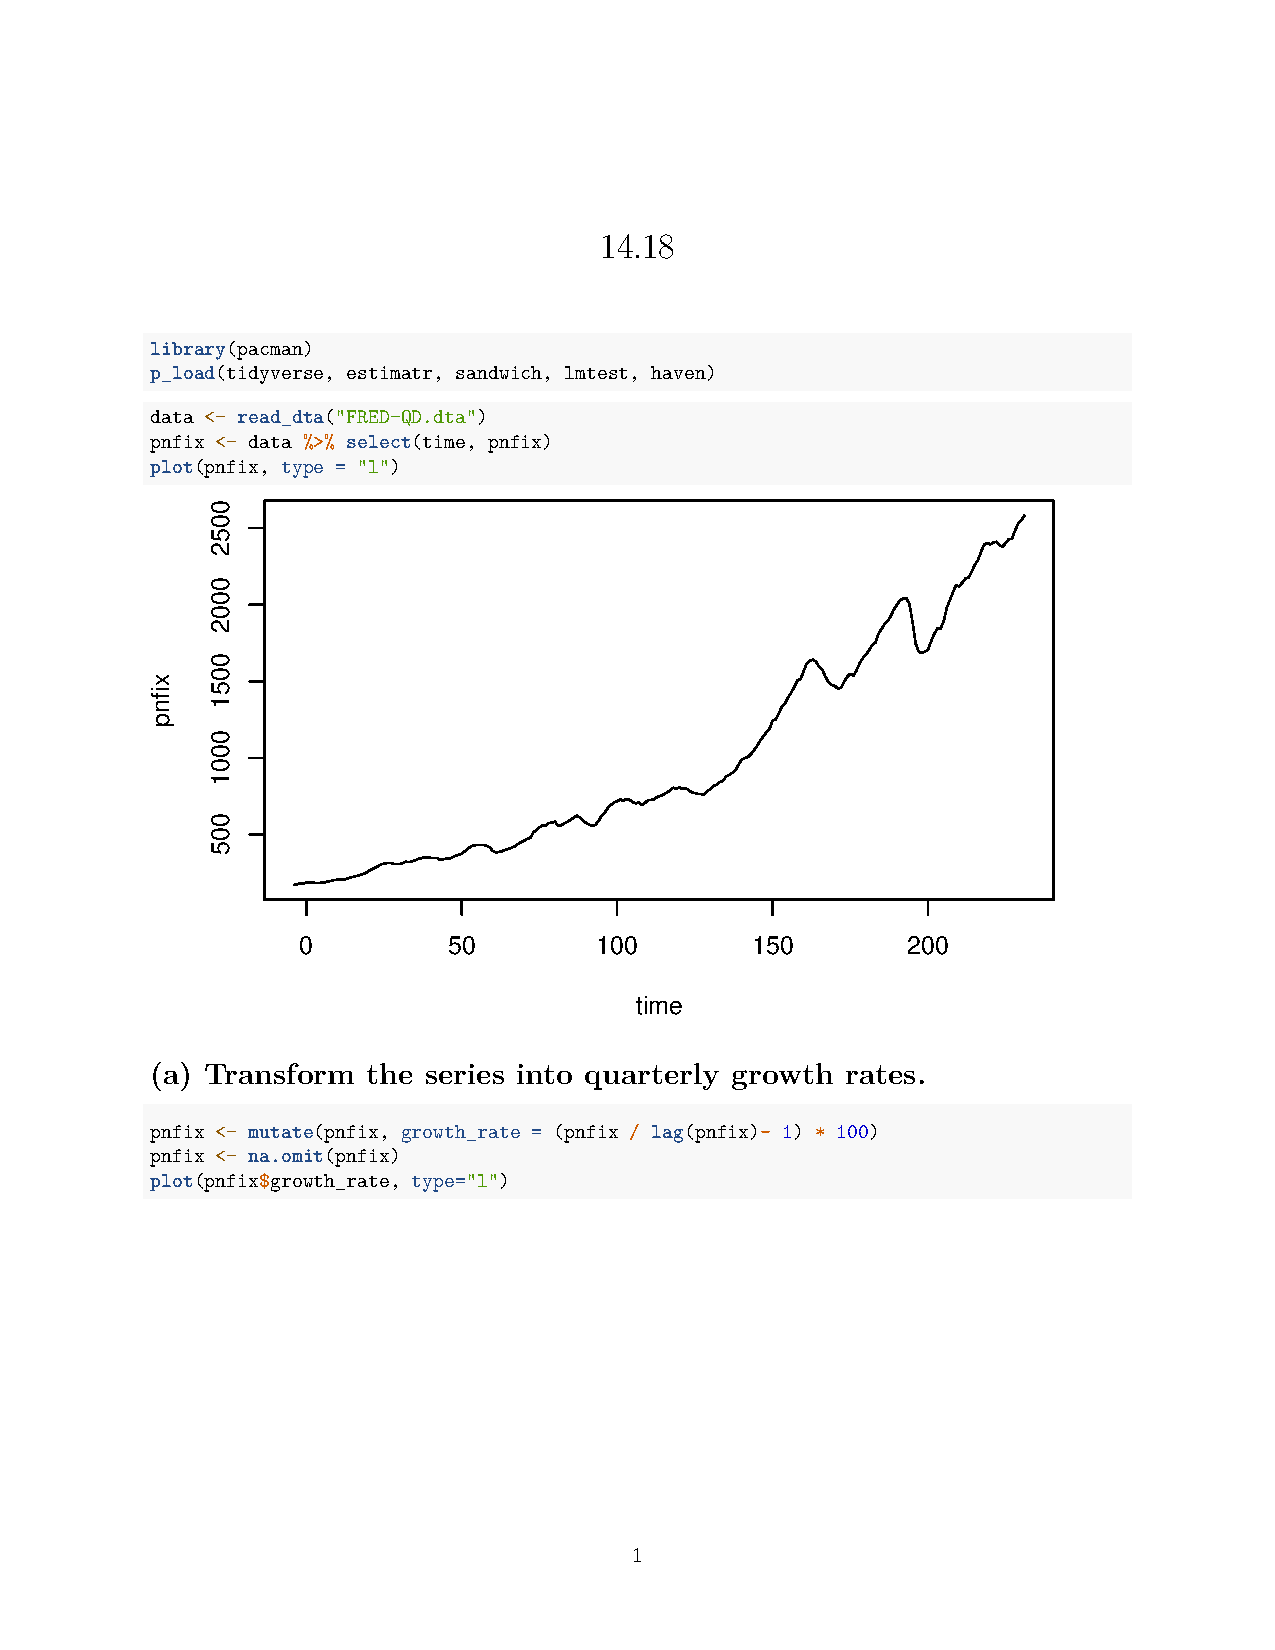
\includepdf[
  pages = - ,        % すべてのページ。1-3 のように範囲指定も可
  pagecommand = {}   % 既存のヘッダ/フッタを消して真っ白に
]{14.18.pdf}

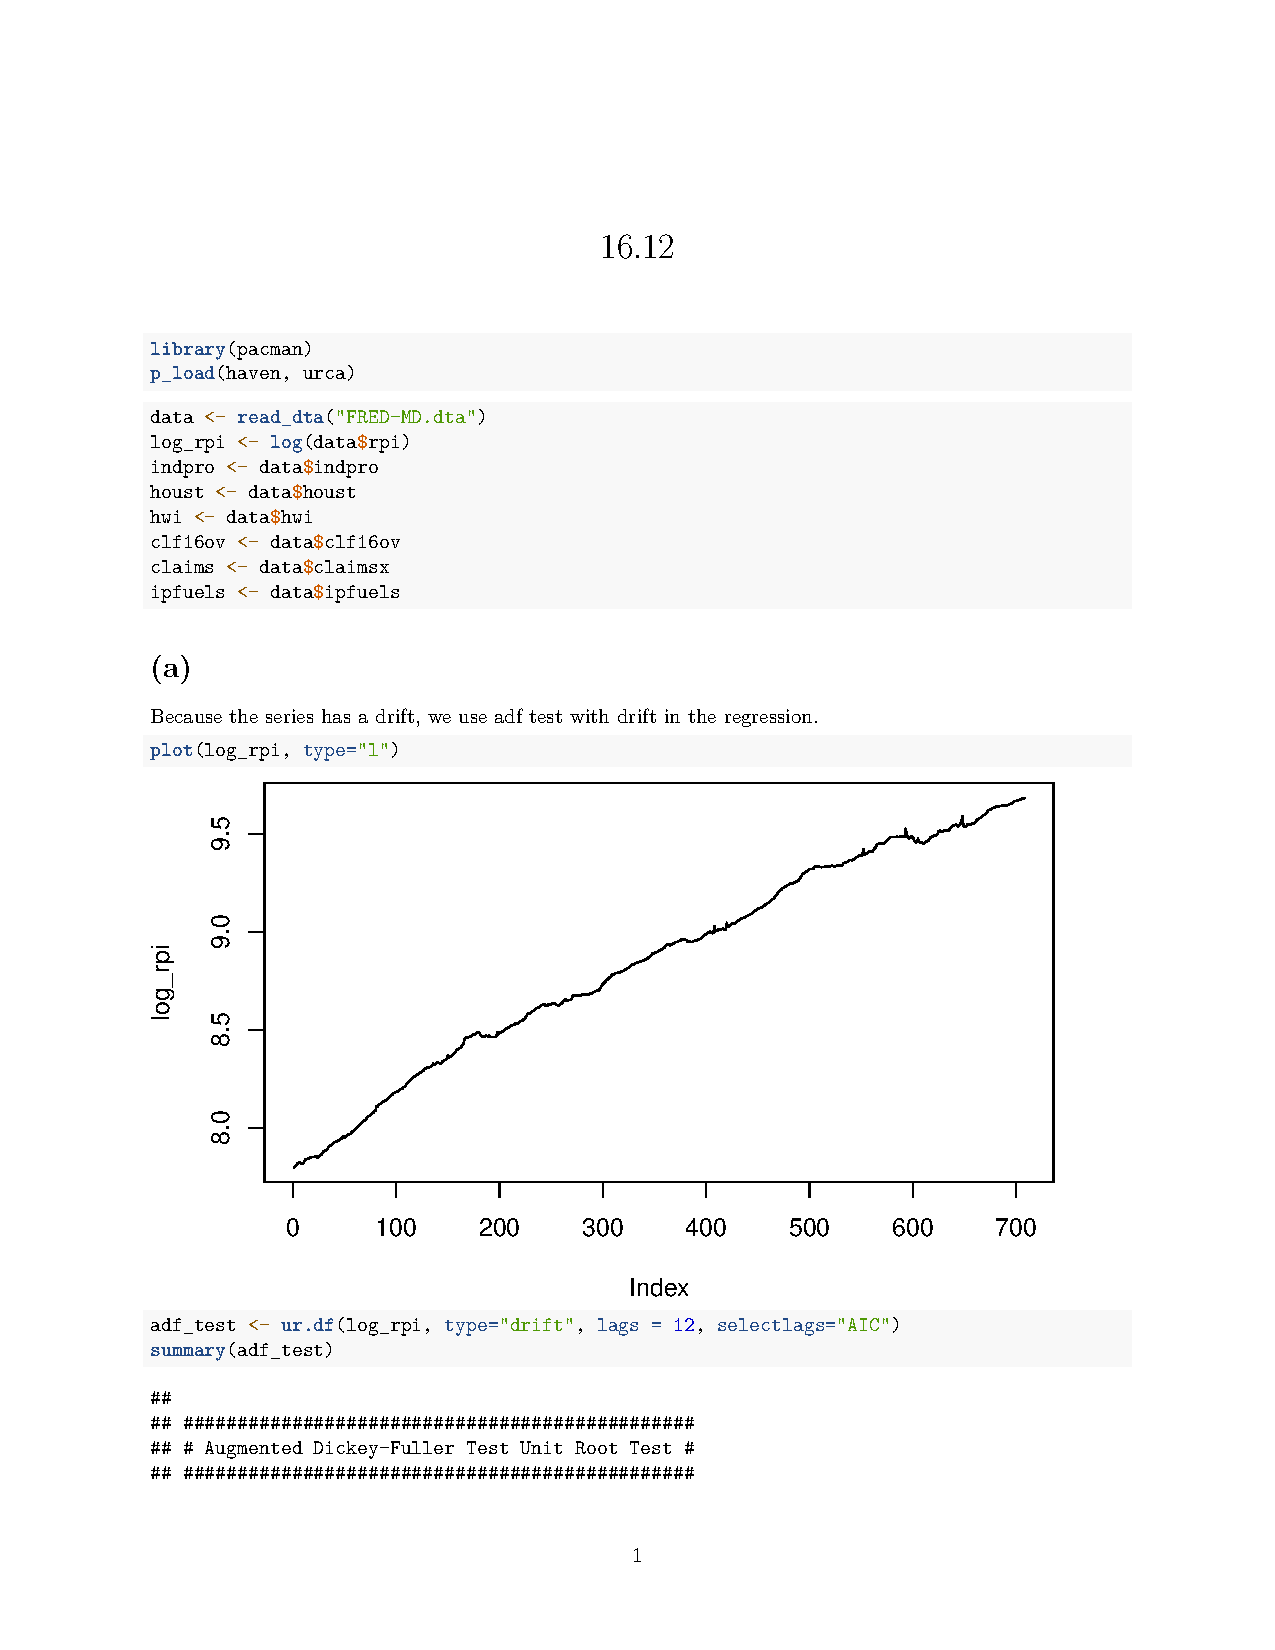
\includepdf[
  pages = - ,        % すべてのページ。1-3 のように範囲指定も可
  pagecommand = {}   % 既存のヘッダ/フッタを消して真っ白に
]{16.12.pdf}

\end{document}
